% !TEX root = ../thesis.tex
% adjust parameter limits
% @author Tobias Wulf
%

\section{Anpassung der Parametergrenzen}\label{sec:exp4}

\textbf{Zweck:}

\textbf{Durchführung:}

\textbf{Erzeugte Datensätze:}

\textbf{Matlab-Skript:}

\textbf{Abweichende Parameter von \autoref{tab:sim-params-exp}:}

Abweichende Parameter:

\begin{itemize}
	\item TrainingsOptions: nAngles: 17
	\item GRPOptions: kernel : 'QFCAPX'
	\item $\sigma_f^2$-Bounds: $(1,10)$
	\item $\sigma_l$-Bounds: $(10,30)$
	\item $\sigma_n^2$-Bounds: $(10^{-6},10^{-4})$
	\item GPROptions: mean: 'zero'
	\item OptimRuns 10
\end{itemize}


\textbf{Ergebnisse:}

Anpassung:

$\sigma_f^2$-Bounds: $(1, 10)$ / $\sigma_l$-Bounds: $(10, 30)$ / $\sigma_n^2$-Bounds: $(10^{-6}, 10^{-4})$
Anpassung: Durchlaufzahl 10

\textbf{Beobachtungen:}


\clearpage
\begin{landscape}
\begin{figure}[tbph]
	\centering
	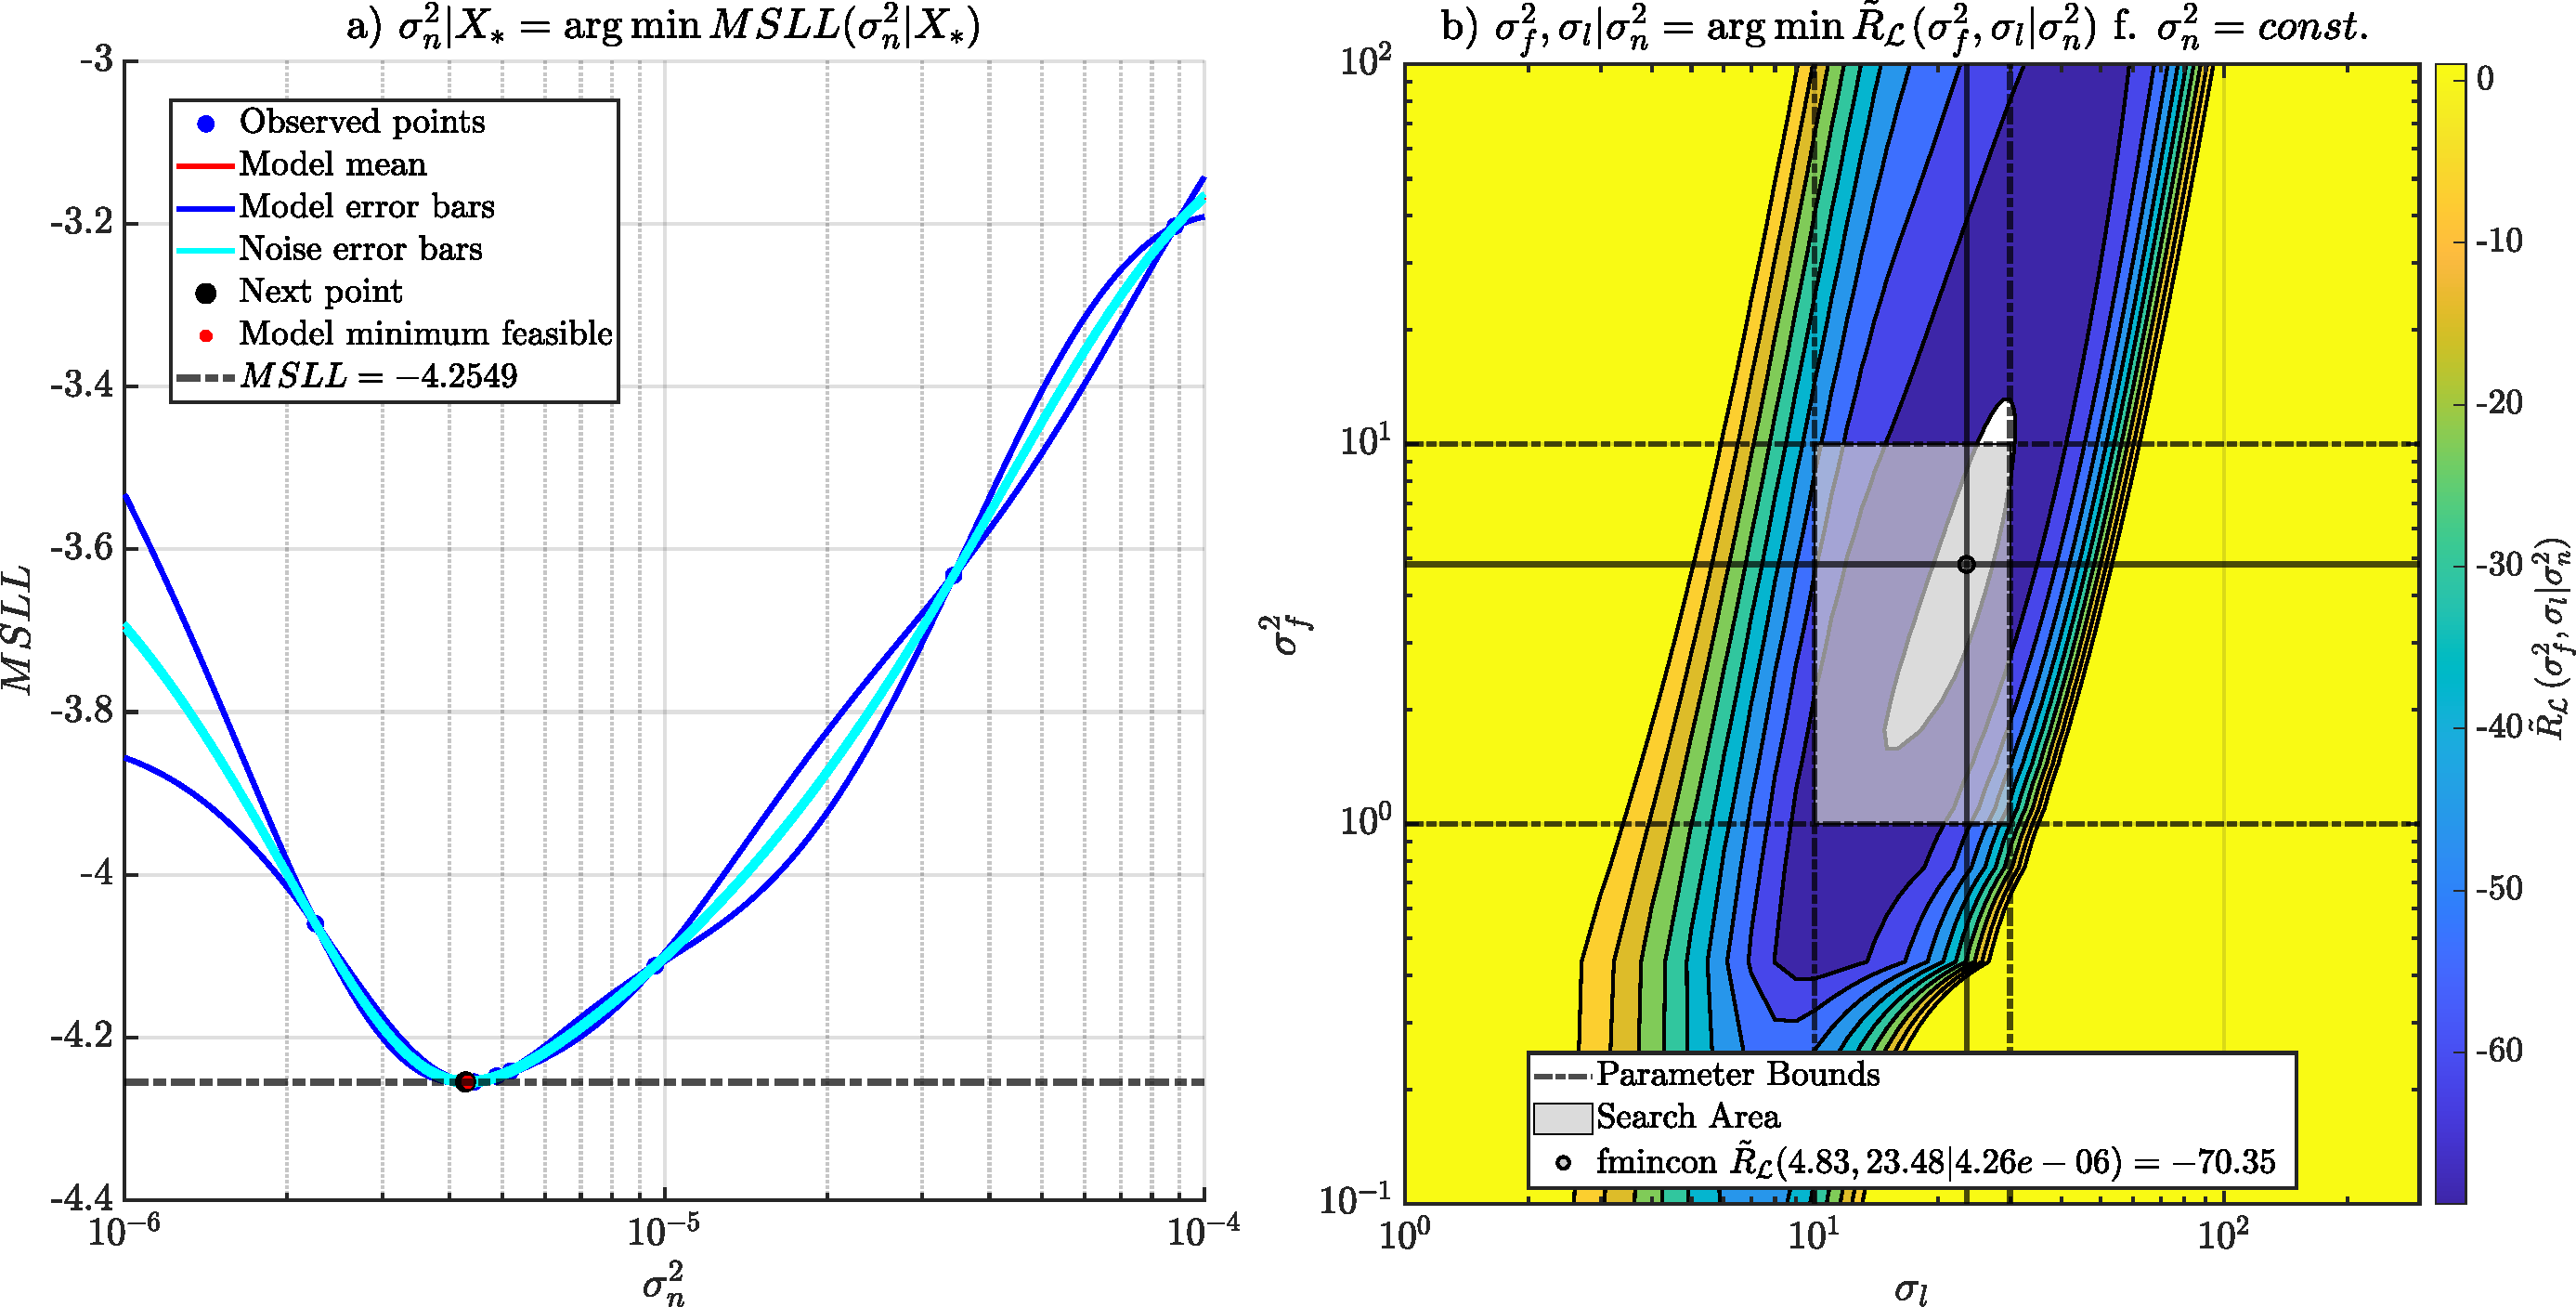
\includegraphics[width=\linewidth]{chapters/images/4-EuOExp/QFCAPX-Z-N17-Bounds}
	\caption[Angepaster Parameter Bounds]{Angepaster Parameter Bounds}
	\label{fig:qfcapx-z-n17-bounds}
\end{figure}
\end{landscape}


\clearpage
\begin{landscape}
\begin{figure}[tbph]
	\centering
	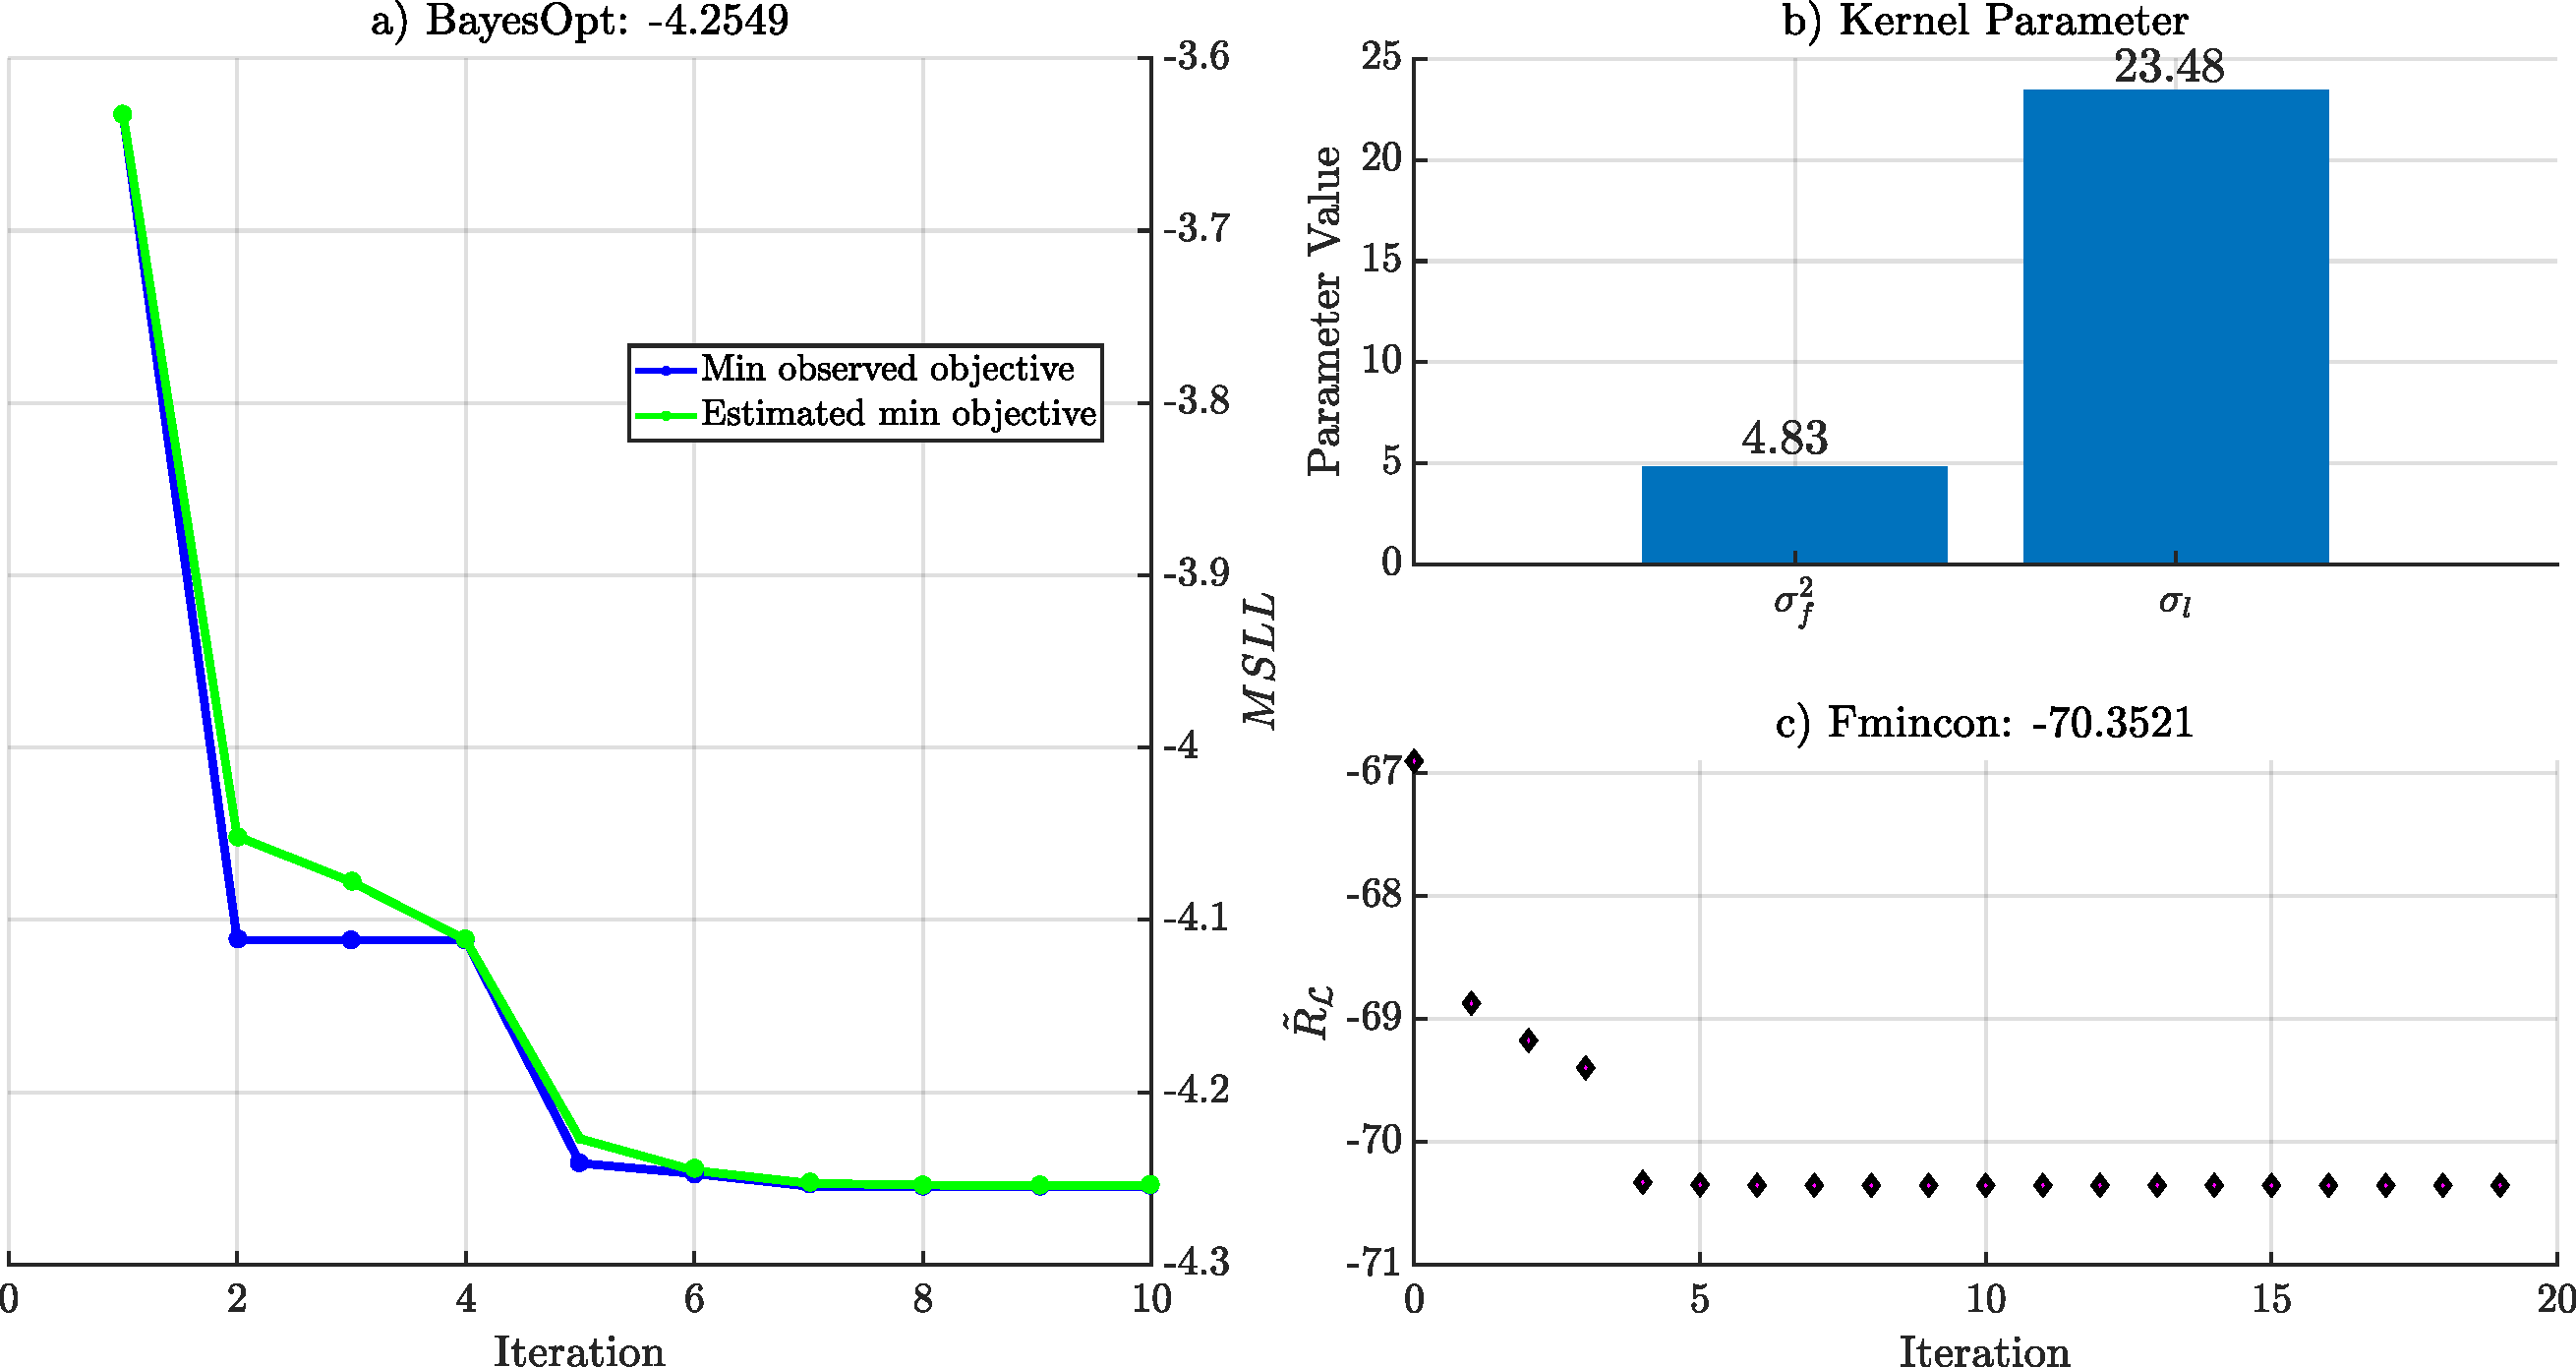
\includegraphics[width=\linewidth]{chapters/images/4-EuOExp/QFCAPX-Z-N17-Opt}
	\caption[QFCAPX Z N17 Optimierung Runs 10]{QFCAPX Z N17 Optimierung Runs 10}
	\label{fig:qfcapx-z-n17-opt}
\end{figure}
\end{landscape}


\clearpage

